\section{Proposed Random Address Translator (RAT)}

From the analysis in the previous sections, it is prominent that the existence of linear correlation between index Bytes of the state matrix and the location of corresponding accessed block in memory is the primary reason of vulnerability of AES in the first round. Given size of memory block (64 Bytes in most of the cases), any information about the memory access during the encryption process would directly reveal high nibble of the index Bytes. Thus if the size of the key is 128 Bit, pre-knowledge of the high nibbles of the index Bytes would reduce the brute force complexity to $2^{64}$.\\

If the correlation can be broken, so that the index Bytes will no longer be used to directly locate the desired block of the Lookup table, most of the cache-timing threats will be eliminated. The key concept to the solution is to perform memory access to get the desired content from an arbitrary, unpredictable location. This can be accomplished by introducing a Translator table between the state matrix and the Lookup table.\\

The most common picture that one might perceive in such a scenario is the mediation of a mapping table that maps one Byte to another. But a flat mapping table would have several disadvantages. First of all, it will incur more cache misses than a normal table lookup encryption process. This may account for disatrous performance concern because cache misses are very expensive. Secondly, it can be large; at least 256 Bytes since the Lookup table itself has 256 entries. A good translator must consume least number of Bytes as part of its mapping operation as well as seek for at most the same number of cache misses that would occur in a normal table lookup operation.\\

One reasonable way to ensure similar number of cache misses as the normal process would be to keep chunks of Bytes of the translator table together and then rearrange them. In our solution, we defined 1 chunk to contain 16 Bytes. So we have a total of 16 chunks and if the memory block (Cache Line) is at least 64 Bytes, it can be easily inferred that we are not incurring more cache misses than the normal process. At present, most processors have 64 Byte cache line.\\

The next big concern is size. Mapping 256 Bytes requires another 256 Bytes, but mapping 256 Bytes with 16 Bytes grouped together requires only 16 Bytes. Let $f(x)$ be that mapping function. Then $f($0x2E$)$ can return anything from the set \{0x0E,0x1E,0x2E,...,0xFE\} but not something like 0x2F or 0xAB. That is, the low nibble will be unchanged.

\begin{center}
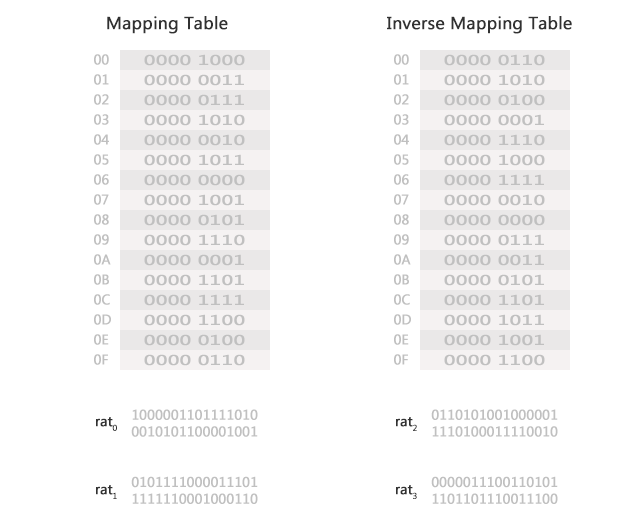
\includegraphics[scale=0.4,natwidth=640,natheight=530]{psd/after.png}
\captionof{figure}{The figure illustrates the state of the mapping and inverse mapping tables after randomization. Since numbers from 0 to 15 requires only 4 bits and a Byte is capable of storing 8 bits, the tables can be condensed by a factor of two and can be conveniently stored as a set of four 32 bit integers $rat_i$ for $0<=i<=3$}
\end{center}

The following algorithm outlines the process. It takes no parameters and returns a set of four integers. The first two integers $rat_0$ and $rat_1$ will be used randomize the Lookup table and the last two integers $rat_2$ and $rat_3$ will be used to retrieve correct piece of information from the Lookup table.

\begin{algorithm}
	\caption{Constructing the RAT}
	\label{Constructing the RAT}

	\begin{algorithmic}[1]
	
	\Function{init}{\null}
	\State $x\gets \{0,1,2,....,15\}$
	\State $y\gets \{0,1,2,....,15\}$
	\State $rat\gets\{0,0,0,0\}$
	\For{Arbitrary number of times}
		\State $i\gets rand() \bmod 16$\Comment{$\bmod$ resembles modulus operation}
		\State $j\gets rand() \bmod 16$
		\State $swap(x_i,x_j)$
		\State $y_{x_j}\gets i$
		\State $y_{x_i}\gets j$
	\EndFor
	\For{$i\gets0$ to $7$}
		\State $rat_0 \gets rat_0 + x_i\ll((7-i)\ll2)$\Comment{$\ll$ resemebles bitwise left shift operation}
		\State $rat_1 \gets rat_1 + x_{i+8}\ll((7-i)\ll2)$
		\State $rat_2 \gets rat_2 + y_i\ll((7-i)\ll2)$
		\State $rat_3 \gets rat_3 + y_{i+8}\ll((7-i)\ll2)$
	\EndFor
	\State delete x,y
	\State return rat
	
	\EndFunction	
	\end{algorithmic}
\end{algorithm}

Now that we have the mapping integers ready, we can proceed to randomize the Lookup table. But for that we need to operate on the integers ($rat_1$ and $rat_2$). The following algorithm does that operation. It takes an offset Byte as argument and returns another offset Byte.

\begin{algorithm}
	\caption{Mapping Fuction}
	\label{Mapping Function}

	\begin{algorithmic}[1]

	\Function{map}{i}
	\If{$((i \mathrel{\&} 128)=0)$}\Comment{$\mathrel{\&}$ resembles bitwise and operation}
		\State $j \gets 0$
	\EndIf
	\State $k \gets ((255-i)\gg 4)\ll 2$\Comment{$\ll$ and $\gg$ resemble bitwise left and right shift operations respectively}
	\State $x \gets (rat_j\gg k)\mathrel{\&} 15$
	\State $y \gets i \mathrel{\&} 15$
	\State return $(x\ll 4)+y$
	\EndFunction

	\end{algorithmic}
\end{algorithm}

To further illustrate what this mapping function does, let us assume that  $map($0x3E$)$ returns 0x9E. This implies that the content of Lookup table at offset 0x9E is now at offset 0x3E. The following $mingle()$ function does the randomization. It takes the original Lookup table as argument and returns the confounded Lookup table. A temporary table is created to make the process really fast. After the randomization is done, that temporary table is completely removed from memory.

\begin{algorithm}
	\caption{Mingling Function}
	\label{Mingling Function}

	\begin{algorithmic}[1]

	\Function{mingle}{table}\Comment{Takes unmodified lookup table as parameter}
	\For{$i \gets 0$ to $255$}
		\For{$j \gets 0$ to $3$}
			\State $temp_{i,j} \gets table_{map(i),j}$
		\EndFor
	\EndFor
	\For{$i \gets 0$ to $255$}
		\For{$j \gets 0$ to $3$}
			\State $table_{i,j} \gets temp_{i,j}$
		\EndFor
	\EndFor
	\State delete $temp$
	\State return $table$
	\EndFunction

	\end{algorithmic}
\end{algorithm}

Now that we have a perplexed Lookup table, encryption can not still be done because the pieces are not in their right place. Here the last two integers $rat_2$ and $rat_3$ comes into action. Their job is to get the correct piece of information from the mixed up Lookup table. For that we need an inverse mapping function. For example, if $map($0x3E$)$ returns 0x9E, $inverseMap($0x9E$)$ would return 0x3E.

\begin{algorithm}
	\caption{Inverse Mapping Fuction}
	\label{Inverse Mapping Function}

	\begin{algorithmic}[1]

	\Function{inverseMap}{i}
	\State $j \gets 3$
	\If{$((i \mathrel{\&} 128)=0)$}\Comment{$\mathrel{\&}$ resembles bitwise and operation}
		\State $j \gets 2$
	\EndIf
	\State $k \gets ((255-i)\gg 4)\ll 2$\Comment{$\ll$ and $\gg$ resemble bitwise left and right shift operations respectively}
	\State $x \gets (rat_j\gg k)\mathrel{\&} 15$
	\State $y \gets i \mathrel{\&} 15$
	\State return $(x\ll 4)+y$
	\EndFunction
	\end{algorithmic}
\end{algorithm}
